\documentclass{article}
\usepackage[utf8]{inputenc}
\usepackage[T1]{fontenc}
\usepackage{graphicx}
\usepackage{amsmath}
\usepackage{blindtext}
\usepackage{fancyhdr}
\usepackage{lastpage}
\usepackage{lscape}

\pagestyle{fancy}
\cfoot{Strona \thepage\ z \pageref{LastPage}}
\renewcommand{\headrulewidth}{0pt}
\fancyhead{}

\begin{document}

\title{AmbulanceServices - specyfikacja implementacyjna}
\author{Aleksandra Kowalczyk, Kacper Seredyn, Kacper Achramowicz}
\date{Grudzień 2020}
\maketitle 
\thispagestyle{fancy}
\renewcommand*\contentsname{Spis treści}


\setcounter{tocdepth}{2}
\tableofcontents

\pagebreak

\section{Opis pakietów}
\subsection{ Pakiet \texttt{reading}}

Pakiet \texttt{reading} jest odpowiedzialny za odczytanie danych z plików, obsługę wyjątków i wyświetlenie odpowiednich komunikatów. Powiązany z pakietami \texttt{gui} i \texttt{main}.

\subsection{ Pakiet \texttt{geometry}}

Pakiet zawiera klasę, która implementuje i obsługuje punkty na mapie. Zawiera metodę odpowiedzialną za wyznaczenie strony wektora, po której znajduje się punkt. Zawiera również implementację wzoru, który wyznacza przecięcia dróg, jego współrzędne i stosunek otrzymanych odcinków.
Pakiet powiązany jest z pakietem main (pobranie danych), i pakietami graph, graham (przekazanie niezbędnych danych, a także informacji o współrzędnych punktów i ich położeniu).
\subsection{Pakiet \texttt{graham}}

Pakiet zawiera implementacje algorytmu Grahama, odpowiedzialnego za wyznaczenie otoczki wypukłej(granic kraju).
Powiązany jest z pakietem  \texttt{geometry} (pobranie danych, metody odpwiedzialne za wyznaczenie położenia punktów względem danych wektorów, informacje o współrzędnych punktów).

\subsection{Pakiet \texttt{graph}}

Pakiet \texttt{graph} zawiera implemntacje algorytmu konstrukcji grafu, który pozwala stworzyć graf szpitali i dróg oraz algorytmu Dijkstry, który wyznacza nakrótsze drogi między punktami. Korzysta z pakietu  \texttt{geometry} (pobranie informacji o drogach, o współrzędnych punktów, przecinania linii,pobranie wyznaczonych granic).

\subsection{Pakiet \texttt{gui}}

Pakiet gui odpowiedzialy jest za obsługę graficzną i zmiany wyglądu ekranu działania programu. Powiązany jest ze wszystkimi pakietami.

\subsection{ Pakiet \texttt{main}}

Pakiet main zawiera reprezentacje obiektu szpital, pacjent i obiekt(pomnik), a także  stanu pacjenta. Pakiet main zawiera klasę odpowiedzialną za uruchomienie programu i wywoływanie kolejnych działań. Powiązany z pakietem reading( pobranie danych z plików), gui i pakietem geometry.


\pagebreak
\section{Opis algorytmów}
\subsection{Alogrytm wyznaczenia, po której stronie wektora znajduje się punkt}
\label{algo_whichside}
Algorytm ten korzysta z utworzonych w algorytmie Grahama wektorów i determinuje, czy dany punkt znajduje się po lewej, czy po prawej stronie każdego z nich. Jeżeli punkt znajduje się po lewej stronie każdego wektora to znaczy, że znajduje się w środku otoczki wypukłej. \\
Używając dwóch punktów leżących na wektorze (A, B) sprawdzamy, czy punkt C leży po lewej stronie wektora przy użyciu poniższego wzoru:

     $${((bX - aX)*(cY - aY) - (bY - aY)*(cX - aX)) > 0}$$

Jeżeli nierówność okaże się prawdziwa, to znaczy, że punkt leży po lewej stronie wektora.

\subsection{Algorytm przecięcia linii (line-line intersection)}
\label{algo_lineline}
    
Algorytm ten określa współrzędne puntku przecięcia linii oraz stosunek w jakim każdy z tych odcinków został podzielony. Korzystamy z lekko zmodyfikowanej wersji oryginalnego algorytmu, ponieważ szukamy punktu przecięcia odcinków, a nie prostych. Z tego względu najpierw zapisujemy linie L1 i L2 w postaci parametrów Béziera pierwszego stopnia, czyli:\\
${\displaystyle L_{1}={x_{1} \choose y_{1}}+t{x_{2}-x_{1} \choose y_{2}-y_{1}},\qquad L_{2}={x_{3} \choose y_{3}}+u{x_{4}-x_{3} \choose y_{4}-y_{3}}}$,\\
\\
gdzie $t$ i $u$ są liczbami rzeczywistymi:\\
\\
$${{\displaystyle t={\frac {\begin{vmatrix}x_{1}-x_{3}&x_{3}-x_{4}\\y_{1}-y_{3}&y_{3}-y_{4}\end{vmatrix}}{\begin{vmatrix}x_{1}-x_{2}&x_{3}-x_{4}\\y_{1}-y_{2}&y_{3}-y_{4}\end{vmatrix}}}={\frac {(x_{1}-x_{3})(y_{3}-y_{4})-(y_{1}-y_{3})(x_{3}-x_{4})}{(x_{1}-x_{2})(y_{3}-y_{4})-(y_{1}-y_{2})(x_{3}-x_{4})}}}}$$

 $${\displaystyle u=-{\frac {\begin{vmatrix}x_{1}-x_{2}&x_{1}-x_{3}\\y_{1}-y_{2}&y_{1}-y_{3}\end{vmatrix}}{\begin{vmatrix}x_{1}-x_{2}&x_{3}-x_{4}\\y_{1}-y_{2}&y_{3}-y_{4}\end{vmatrix}}}=-{\frac {(x_{1}-x_{2})(y_{1}-y_{3})-(y_{1}-y_{2})(x_{1}-x_{3})}{(x_{1}-x_{2})(y_{3}-y_{4})-(y_{1}-y_{2})(x_{3}-x_{4})}},}$$


Wtedy współrzędne punktu przecięcia znajdujemy według jednego ze wzorów: 
${\displaystyle (P_{x},P_{y})=(x_{1}+t(x_{2}-x_{1}),\;y_{1}+t(y_{2}-y_{1}))}\quad $\\
$\displaystyle\quad (P_{x},P_{y})=(x_{3}+u(x_{4}-x_{3}),\;y_{3}+u(y_{4}-y_{3}))\quad$

Jeżeli t >= 0 i t <= 1 to wtedy punkt przecięcia przypada na pierwszy odcinek, natomiast gdy u >= 0 i u <= 1.
\subsection{Algorytm konstrukcji grafu}
\label{algo_graphconstr}

Aby utworzyć graf szpitali oraz dróg je łączących, należy najpierw odpowiednio dokonać obróbki surowych danych połączeń - przecięcia odcinków dróg powinny skutkować utworzeniem skrzyżowań. \\
Algorytm konstrukcji grafu działa przy poniższych założeniach:

\begin{itemize}
    \item Linie połączeń dodawane są do algorytmu pojedynczo,
    \item Algorytm sprawdza interakcje nowych linii z liniami już odpowiednio przeciętymi.
\end{itemize}

Dzięki powyższym obostrzeniom, algorytm może przyjąć postać iteracyjną, wykonywaną dla każdego odcinka drogi w systemie:

\begin{enumerate}
    \item \emph{Obliczenie przecięć z liniami już przetworzonymi:} \\
          \centerline{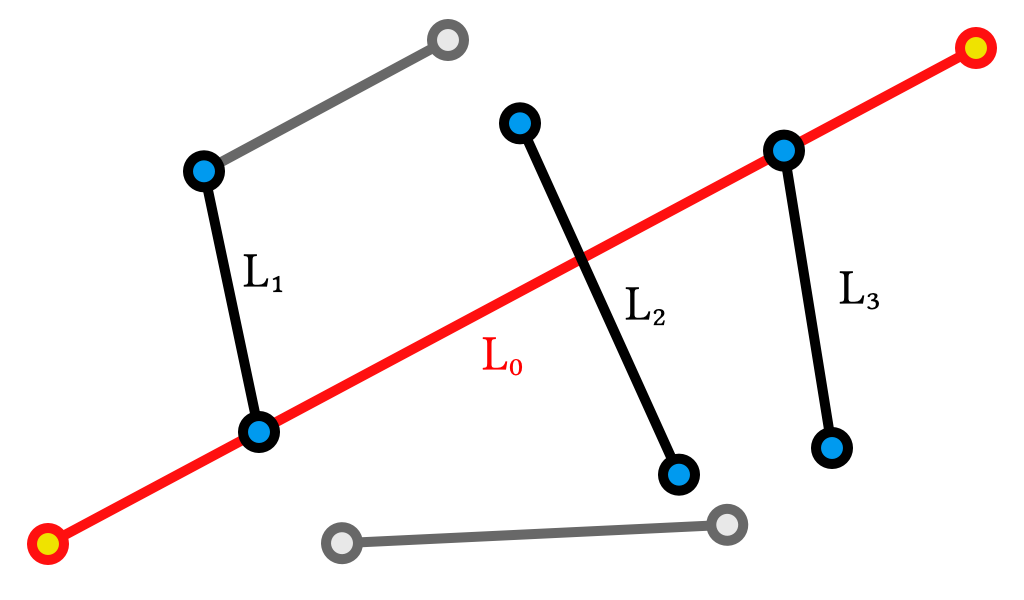
\includegraphics[scale=0.3]{images/line1.png}}
          
          Przy użyciu algorytmu z sekcji \ref{algo_lineline}, znajdywane są linie, które się przecinają z drogą tnącą (zaznaczoną na czerwono), wraz z pozycjami \((t, u)\) punktu przecięcia:
          \begin{itemize}
              \item \(t\) - pozycja punktu przecięcia na drodze tnącej,
              \item \(u\) - pozycja punktu przecięcia na drodze ciętej.
          \end{itemize}
          
\pagebreak
    \item \emph{Tworzenie nowych dróg:} \\
          \centerline{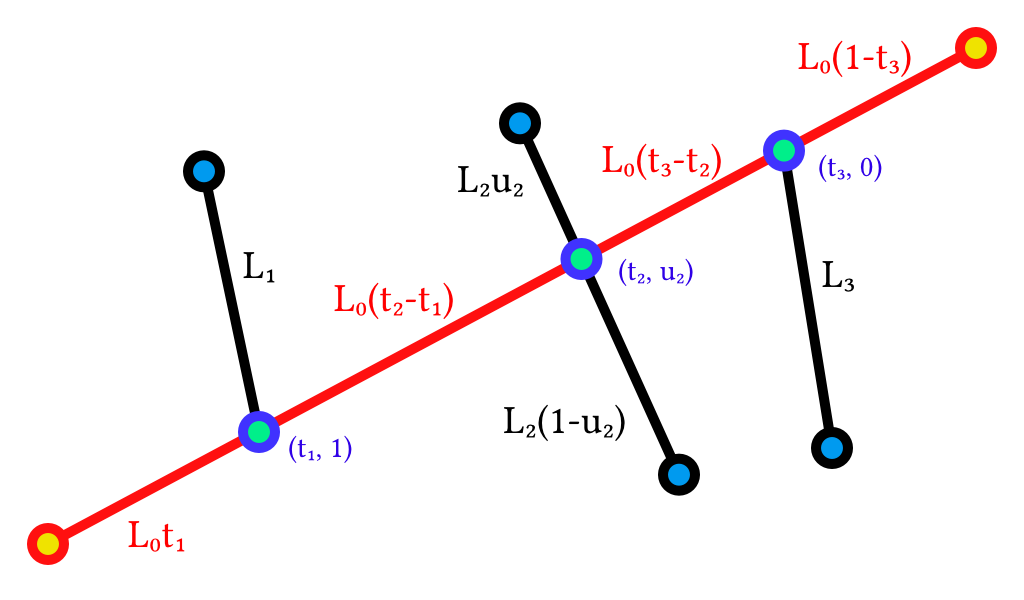
\includegraphics[scale=0.3]{images/line2.png}}
          
          Na podstawie wartości \((t, u)\) tworzone są nowe drogi o odpowiednio obliczonych długościach (jak na powyższym diagramie). W przypadku, gdy wartość \(u\) nie jest równa 0 lub 1, tworzony jest dodatkowy punkt skrzyżowania.
\end{enumerate}

\subsection{Algorytm Dijkstry}
\label{algo_dijkstra}
Do wyznaczenia najkrótszych dróg między szpitalami, program używa algorytmu grafowego Dijsktry:

\begin{enumerate}
    \item \emph{Przygotowanie algorytmu}: \\
          Przed rozpoczęciem iteracji po węzłach grafu, konieczne jest przygotowanie kilku zmiennych i dokonanie pewnych operacji:
          \begin{itemize}
                \item V[n] - tablica wszystkich n węzłów grafu,
                \item S - węzeł źródłowy,
                \item D[n] - tablica odległości n węzłów od węzła S. \\
                    Wszystkie wartości tablicy D są zainicjalizowane na dodatnią nieskończoność, poza D[j] = 0, dla takiego j, gdzie V[j] = S.
                \item P[n] - tablica poprzedników. \\
                    Wszystkie wartości tablicy P są zainicjalizowane na \texttt{null}.
                \item Wszystkie węzły grafu zostają odznaczone (\texttt{Graph.setAllMarks}).
          \end{itemize}
    \item \emph{Iteracja po V[n]}:
          \begin{enumerate}
              \item Pobierany jest \emph{nieoznaczony} węzeł V[i] = N o najmniejszej wartości D[i]. Jest on następnie oznaczany (\texttt{Graph.setMark}).
              \item Dla każdego nieoznaczonego sąsiada V[j] = P węzła N obliczana jest nowa odległość: \({L = D[i] + len(N, P)}\), gdzie len(A, B) - długość krawędzi łączącej A i B. \\
                    Jeśli \(L < D[j]\), to \(D[j] = L\) i \(P[j] = N\).
              \item Jeśli pozostały w grafie nieoznaczone węzły, powrót to kroku pierwszego iteracji.
          \end{enumerate}
\end{enumerate}


\subsection{Algorytm Grahama}
\label{algo_graham}

Algorytm Grahama służy do znajdowania otoczki wypukłej. Na początku znajduje punkt najbardziej wysunięty na lewo. Jeżeli jest kilka takich punktów wybiera punkt znajdujący się najbardziej na dole. Jest to tzw. punkt bazowy. Kolejne punkty są sortowane względem kątów nachylenia ich wektorów względem osi, którą w płaszczyźnie x tworzy punkt startowy.
Algorytm przechodząc od punktu startowego do kolejnych punktów z posortowanej listy,umieszcza je na stosie i sprawdza kierunek, w którym nastąpiło to przejście:
\begin{itemize}
 \item jeżeli odchylenie nastąpiło w prawą stronę, zdejmowany jest wierzchołek ze stosu
 \item jeżeli odchylenie nastąpiło w stronę lewą, wierzchołek pozostaje na stosie
\end{itemize}
Finalnie otrzymujemy stos, który zawiera jedynie te punkty, które tworzą otoczkę wypukłą.

\pagebreak
\section{Opis graficznego interfejsu użytkownika}

\centerline{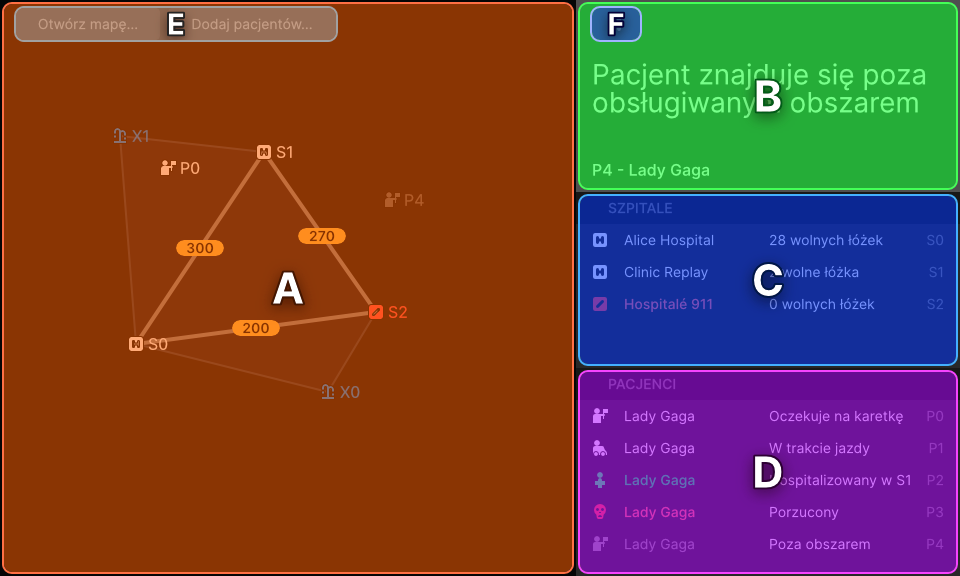
\includegraphics[scale=0.3]{images/areas.png}}

 \vspace{0.7cm}
 
\begin{itemize}
    \item A - mapa szpitali, obiektów i położeń pacjentów,
    \item B - sekcja informacyjna,
    \item C - lista szpitali,
    \item D - lista pacjentów,
    \item E - przyciski ładowania plików,
    \item F - przycisk kontroli symulacji ("Uruchom"/"Wstrzymaj")
\end{itemize}

\subsection{Przyciski \emph{ładowania plików}}
\label{gui_filebuttons}
Słuchaczem przycisku "Otwórz mapę..." i "Dodaj pacjentów..." jest klasa reading.Reader która pobiera i przetwarza dane z pliku mapy i pliku pacjenci. Wynikiem naciśnięcia przycisku są pola "Mapa szpitali, obiektów i pacjentów", "Lista szpitali", "Lista pacjentów".

\subsection{Przyciski \emph{kontroli symulacji}}
Przyciski "Uruchom"/"Wstrzymaj" służą do rozpoczęcia/ wstrzymania działania przeprowadzania symulacji. Słuchaczami przycisków jest klasa odpowiedzialna na rysowanie na ekranie kolejnych stanów obsługi pacjenta.

\subsection{Pole \emph{Mapa szpitali, obiektów i położeń pacjentów}}
\label{gui_map}
W tym polu wyświetlana jest mapa, zawierająca wyznaczoną otoczkę wypukłą, obiekty, szpitale, drogi między nimi wraz z ich odległościami, skrzyżowania i oznaczenia pacjentów wraz z ich aktualnym stanem. Słuchaczami tego pola są klasy z pakietu graph, geometry, graham.

\subsection{Pole \emph{Sekcja informacyjna}}
\label{gui_info}
Pole wyświetla infomacje o aktualnym stanie obsługi danego pacjenta. Słuchaczem pola jest klasa main.Patient oraz klasa main.State.

\subsection{Pole \emph{Lista szpitali}}
\label{gui_hospital}
Słuchaczem pola jest klasa main.Hospital. W tym polu wyświetlane są nazwy szpitali, liczba dostępnych wolnych łóżek,która na bieżąco jest aktualizowana i skrót, którymi oznaczone są na mapie.

\subsection{Pole \emph{Lista pacjentów}}
\label{gui_patients}
Słuchaczem pola jest klasa Patient. W tym polu wyświetlane są id pacjentów, stan przyjęcia, który jest na bieżąco aktualizowany i skrót, którymi oznaczeni są na mapie.

\label{gui_start_stop}

\pagebreak
\section{Opis klas}

Poniżej znajduje się lista pól i metod klas projektu. Diagram UML klas znajduje się na końcu rozdziału.

\subsection{Klasa \texttt{reading.Reader}}
Wczytuje dane z pliku do programu.

\subsubsection{Pole \texttt{Reader.Parser}}
\texttt{private final Parser parser} \\
Obiekt \texttt{Parser}.

\subsubsection{Metoda \texttt{Reader.load}}
\texttt{public State load(String fileName)} \\
Wczytuje dane z pliku, którego nazwa została podana jako argument wywołania.

\subsection{Klasa \texttt{reading.Parser}}
Zajmuje się obróbką danych przekazanych do programu.

\subsubsection{Metoda \texttt{Parser.parseHospital}}
\texttt{public void parseHospital(State state, String[] buffer)} \\
Tworzy obiekt \texttt{Hospital} na podstawie argumentu \texttt{buffer} i dodaje go do listy szpitali w \texttt{state}.

\subsubsection{Metoda \texttt{Parser.parseLandmark}}
\texttt{public void parseLandmark(State state, String[] buffer)} \\
Tworzy obiekt \texttt{Landmark} na podstawie argumentu \texttt{buffer} i dodaje go do listy obiektów w \texttt{state} .

\subsubsection{Metoda \texttt{Parser.parsePatient}}
\texttt{public void parsePatient(State state, String[] buffer)} \\
Tworzy obiekt \texttt{Patient} na podstawie argumentu \texttt{buffer} i dodaje go do listy pacjentów w \texttt{state}. 

\subsubsection{Metoda \texttt{Parser.parseConnection}}
\texttt{public void parseConnection(State state, String[] buffer)} \\
Tworzy obiekt \texttt{Connection} na podstawie argumentu \texttt{buffer}. i dodaje go do listy połączeń w \texttt{state}. 

\pagebreak
\subsection{Klasa \texttt{geometry.LineIntersection}}
Przechowuje metody pozwalające na wyznaczenie punktu przecięcia linii i stosunku, w jakim zostały te linie podzielone.

\subsubsection{Metoda \texttt{LineIntersection.intersect}}
\texttt{public double[] intersect} \\
Metoda jest implementacją algorytmu przecięcia linii.

\subsection{Klasa \texttt{geometry.Point}}
Klasa będąca bazą dla klas Hospital, Patient i Landmark. Zawiera metody pozwalające pobrać informacje punktach na mapie.

\subsubsection{Pole \texttt{Point.x}}
\texttt{private double x} \\
Przechowuje wartość współrzędnej X punktu.

\subsubsection{Pole \texttt{Point.y}}
\texttt{private double y} \\
Przechowuje wartość współrzędnej Y punktu.

\subsubsection{Konstruktor \texttt{Point}}
\texttt{public Point(double x, double y)} \\
Tworzy obiekt \texttt{Point} o podanych współrzędnych.

\subsubsection{Konstruktor \texttt{Point}}
\texttt{public Point(double x, Point start, Point end)} \\
Tworzy obiekt \texttt{Point} w miejscu wyznaczonym przez proporcję \texttt{x} na odcinku utworzonym przez dwa \texttt{punkty}.

\subsubsection{Metoda \texttt{Point.getRelativeDirection}}
\texttt{public double getRelativeDirection()} \\
Zwraca wartość potrzebną do wyznaczenia, po której stronie wektora znajduje się punkt (algorytm \ref{algo_whichside}).

\subsubsection{Metoda \texttt{Point.getX}}
\texttt{public double getX()} \\
Zwraca wartość współrzędnej X.

\subsubsection{Metoda \texttt{Point.getY}}
\texttt{public double getY()} \\
Zwraca wartość współrzędnej Y.

\subsubsection{Metoda \texttt{Point.isLeft}}
\texttt{public boolean isLeft()} \\
Implementuje algorytm wyznaczenia, po której stronie wektora znajduje się punkt (algorytm \ref{algo_whichside}).

\pagebreak
\subsection{Klasa \texttt{graham.ConvexHull}}
Reprezentuje otoczkę wypukłą.

\subsubsection{Konstruktor \texttt{ConvexHull}}
\texttt{public ConvexHull(List<Point> points)} \\
Tworzy obiekt \texttt{ConvexHull} na podstawie danej listy punktów otoczki.

\subsubsection{Pole \texttt{ConvexHull.points}}
\texttt{private List<Points> points} \\
Lista punktów otoczki wypukłej.

\subsubsection{Metoda \texttt{ConvexHull.chooseStartPoint}}
\texttt{public Point chooseStartPoint(Point point)} \\
Zwraca punkt \texttt{Point StartPoint}, którego współrzędna x jest najmniesza. W przypadku gdy jest kilka punktów o tej samej współrzędnej x wybiera punkt o najmniejszej wartości y.


\subsubsection{Metoda \texttt{ConvexHull.calculateAngles}}
\texttt{public double[] calculateAngles(Point startPoint, List<Point> points)} \\
Oblicza wartości kątowe między punktem startowym ( osią x wyznaczoną przez punkt startowy) a pozostałymi punktami. Zwraca tablice zawierającą wartość kątową dla każdego punktu.

\subsubsection{Metoda \texttt{ConvexHull.sortByAngles}}
\texttt{public List<Point> sortByAngles(List<Point> points, double[] angles)} \\
Zwraca posortowaną listę puntów \texttt{List<Point> sortedPoints} od najmniejszej do największej wartości kątowej.

\subsubsection{Metoda \texttt{ConvexHull.isPointInHull}}
\texttt{public boolean isPointInHull(Point point)} \\
Zwraca \texttt{true} jeśli punkt \texttt{point} znajduje się wewnątrz otoczki wypukłej, w przeciwnym wypadku zwraca \texttt{false}.

\pagebreak
\subsection{Klasa \texttt{graph.Graph<T>}}
Przechowuje graf nieskierowany.

\subsubsection{Konstruktor \texttt{Graph}}
\texttt{public Graph()} \\
Tworzy obiekt \texttt{Graph}.

\subsubsection{Pole \texttt{Graph.edges}}
\texttt{private Double[][] edges} \\
Macierz połączeń węzłów grafu. \\
Jeśli wartość \(edges[i][j]\) jest równa \texttt{null}, między wierzchołkami \(i\) i \(j\) nie ma połączenia. W przeciwnym razie, liczba w \(edges[i][j]\) jest długością połączenia między \(i\) i \(j\).

\subsubsection{Pole \texttt{Graph.marks}}
\texttt{private List<boolean> marks} \\
Lista oznaczeń węzłów grafu. Oznaczenia używane są przez algorytm Dijkstry (\ref{algo_dijkstra}).

\subsubsection{Pole \texttt{Graph.nodes}}
\texttt{private List<T> nodes} \\
Lista węzłów grafu.

\subsubsection{Metoda \texttt{Graph.addNode}}
\texttt{public int addNode(T node)} \\
Dodaje węzeł do grafu i zwraca ilość węzłów po dodaniu.

\subsubsection{Metoda \texttt{Graph.connectNodes}}
\texttt{public void connectNodes(T n1, T n2, double length)} \\
Łączy dwa węzły grafu połączeniem o długości \texttt{length}.

\subsubsection{Metoda \texttt{Graph.finalizeNodes}}
\texttt{public void finalizeNodes()} \\
Tworzy tablicę \texttt{Double[][] edges} o wymiarach \([n][n]\) (\(n\) - liczba węzłów) zainicjalizowaną wartościami \texttt{null}.

\subsubsection{Metoda \texttt{Graph.getLength}}
\texttt{public Double getLength(T n1, T n2)} \\
Zwraca długość połączenia między węzłami \texttt{n1} i \texttt{n2} lub \texttt{null} jeśli połączenie nie istnieje.

\subsubsection{Metoda \texttt{Graph.getMark}}
\texttt{public boolean getMark(T node)} \\
Zwraca wartość oznaczenia węzła \texttt{node}.

\subsubsection{Metoda \texttt{Graph.getNeighbors}}
\texttt{public List<T> getNeighbors(T node)} \\
Zwraca sąsiadów węzła \texttt{node} (węzłów połączonych do węzła \texttt{node}).

\subsubsection{Metoda \texttt{Graph.getNodes}}
\texttt{public List<T> getNodes(Boolean mark = null)} \\
Zwraca węzły w grafie. Jeśli wartość \texttt{mark} nie jest \texttt{null}, zwracane są jedynie węzły o oznaczeniu \texttt{mark}.

\subsubsection{Metoda \texttt{Graph.getPathLength}}
\texttt{public double getPathLength(List<T> path)} \\
Zwraca długość ścieżki na podstawie listy węzłów w ścieżce.

\subsubsection{Metoda \texttt{Graph.setAllMarks}}
\texttt{public void setAllMarks(boolean mark)} \\
Ustawia oznaczenia wszystkich węzłów na \texttt{mark}.

\subsubsection{Metoda \texttt{Graph.setMark}}
\texttt{public void setMark(T node, boolean mark)} \\
Ustawia oznaczenia wszystkich węzła \texttt{node} na \texttt{mark}.

\subsection{Klasa \texttt{graph.DijkstraAlgorithm<T>}}
Pozwala na wykonanie algorytmu Dijkstry na grafie.

\subsubsection{Konstruktor \texttt{DijkstraAlgorithm}}
\texttt{public DijkstraAlgorithm(Graph<T> graph)} \\
Tworzy obiekt \texttt{DijkstraAlgorithm} dla danego grafu.

\subsubsection{Pole \texttt{DijkstraAlgorithm.distances}}
\texttt{private Double[] distances} \\
Tablica odległości w grafie (algorytm \ref{algo_dijkstra}).

\subsubsection{Pole \texttt{DijkstraAlgorithm.graph}}
\texttt{private Graph graph} \\
Graf, na którym działa algorytm.

\subsubsection{Pole \texttt{DijkstraAlgorithm.previousNodes}}
\texttt{private T[] previousNodes} \\
Tablica poprzedników węzłów grafu (algorytm \ref{algo_dijkstra}).

\subsubsection{Metoda \texttt{DijkstraAlgorithm.getNextNode}}
\texttt{private T getNextNode()} \\
Zwraca kolejny węzeł do przetwarzania w algorytmie (algorytm \ref{algo_dijkstra}).

\subsubsection{Metoda \texttt{DijkstraAlgorithm.iterateOverNeighbors}}
\texttt{private void iterateOverNeighbors(T node)} \\
Dokonuje iteracji algorytmu po danym węźle (algorytm \ref{algo_dijkstra}).

\subsubsection{Metoda \texttt{DijkstraAlgorithm.execute}}
\texttt{private void execute(T source)} \\
Uruchamia algorytm dla węzła startowego \texttt{source} (algorytm \ref{algo_dijkstra}).

\subsubsection{Metoda \texttt{DijkstraAlgorithm.getPath}}
\texttt{private List<T> getPath(T target)} \\
Zwraca ścieżkę z węzła zdefiniowanego przy wywołaniu \texttt{execute()} a  \texttt{target} (alogrytm \ref{algo_dijkstra}). Jeśli ścieżka nie istnieje, zwraca \texttt{null}.

\subsection{Klasa \texttt{graph.GraphConstructorLine}}
Odcinek drogi między dwoma punktami na mapie.

\subsubsection{Konstruktor \texttt{GraphConstructorLine}}
\texttt{public GraphConstructorLine(Point start, Point end, double length)} \\
Tworzy obiekt \texttt{GraphConstructorLine} dla danej drogi.

\subsubsection{Pole \texttt{GraphConstructorLine.end}}
\texttt{private Point end} \\
Punkt końcowy drogi.

\subsubsection{Pole \texttt{GraphConstructorLine.length}}
\texttt{private double length} \\
Długość drogi (niekoniecznie na podstawie odległości euklidesowej między punktami).

\subsubsection{Pole \texttt{GraphConstructorLine.start}}
\texttt{private Point start} \\
Punkt początkowy drogi.

\subsubsection{Metoda \texttt{GraphConstructorLine.getEnd}}
\texttt{public Point getEnd()} \\
Zwraca punkt końcowy drogi.

\subsubsection{Metoda \texttt{GraphConstructorLine.getLength}}
\texttt{public double getLength()} \\
Zwraca długość drogi.

\subsubsection{Metoda \texttt{GraphConstructorLine.getStart}}
\texttt{public Point getStart()} \\
Zwraca punkt początkowy drogi.

\subsection{Klasa \texttt{graph.GraphConstructorCut}}
Przechowuje informacje o przecięciu drogi.

\subsubsection{Konstruktor \texttt{GraphConstructorCut}}
\texttt{public GraphConstructorCut(GraphConstructorLine line, double linePosition, double cutterPosition)} \\
Tworzy obiekt \texttt{GraphConstructorCut} na podstawie informacji o przecięciu.

\subsubsection{Pole \texttt{GraphConstructorCut.cutterPosition}}
\texttt{private double cutterPosition} \\
Pozycja punktu przecięcia na przecinającej linii w zakresie \([0-1]\).

\subsubsection{Pole \texttt{GraphConstructorCut.line}}
\texttt{private GraphConstructorLine line} \\
Przecinana linia grafu.

\subsubsection{Pole \texttt{GraphConstructorCut.linePosition}}
\texttt{private double linePosition} \\
Pozycja punktu przecięcia na przecinanej linii w zakresie \([0-1]\).

\subsubsection{Metoda \texttt{GraphConstructorCut.getCutterPosition}}
\texttt{public double getCutterPosition()} \\
Zwraca pozycję punktu przecięcia na przecinającej linii w zakresie \([0-1]\).

\subsubsection{Metoda \texttt{GraphConstructorCut.getLine}}
\texttt{public GraphConstructorLine getLine()} \\
Zwraca przecinaną linię grafu.

\subsubsection{Metoda \texttt{GraphConstructorCut.getLinePosition}}
\texttt{public double getLinePosition()} \\
Zwraca pozycję punktu przecięcia na przecinanej linii w zakresie \([0-1]\).

\subsection{Klasa \texttt{graph.GraphConstructor}}
Pozwala na utworzenie grafu na podstawie informacji o przecinających się drogach.

\subsubsection{Pole \texttt{GraphConstructor.lines}}
\texttt{private List<GraphConstructorLine> lines} \\
Lista już przetworzonych linii (algorytm \ref{algo_graphconstr}).

\subsubsection{Pole \texttt{GraphConstructor.points}}
\texttt{private Set<Point> points} \\
Zbiór punktów grafu.

\subsubsection{Metoda \texttt{GraphConstructor.cutLines}}
\texttt{private void cutLines(GraphConstructorLine cutter, List<GraphConstructorCut> lines)} \\
Tworzy skrzyżowania dróg i oblicza nowe długości odcinków (algorytm \ref{algo_graphconstr}).

\subsubsection{Metoda \texttt{GraphConstructor.findIntersections}}
\texttt{private List<GraphConstructorCut> findIntersections(GraphConstructorLine cutter)} \\
Znajduje kolizje dróg i tworzy listę przecinanych dróg (algorytm \ref{algo_graphconstr} oraz \ref{algo_lineline}).

\subsubsection{Metoda \texttt{GraphConstructor.addLine}}
\texttt{public void addLine(Point start, Point end, double length)} \\
Dodaje linię do algorytmu.

\subsubsection{Metoda \texttt{GraphConstructor.constructGraph}}
\texttt{public Graph<Point> constructGraph()} \\
Generuje ostateczny graf.

\pagebreak
\subsection{Klasa \texttt{main.Hospital}}
Reprezentuje obiekt szpitala. \\
Klasa \texttt{Hospital} dziedziczy po klasie \texttt{Point}.

\subsubsection{Konstruktor \texttt{Hospital}}
\texttt{public Hospital(int id, double x, double y, String name, int vacantBeds)} \\
Tworzy obiekt \texttt{Hospital}.

\subsubsection{Pole \texttt{Hospital.id}}
\texttt{private int id} \\
Identyfikator szpitala.

\subsubsection{Pole \texttt{Hospital.name}}
\texttt{private String name} \\
Nazwa szpitala.

\subsubsection{Pole \texttt{Hospital.vacantBeds}}
\texttt{private int vacantBeds} \\
Liczba wolnych łóżek.

\subsubsection{Metoda \texttt{Hospital.getId}}
\texttt{public int getId()} \\
Zwraca identyfikator szpitala.

\subsubsection{Metoda \texttt{Hospital.getName}}
\texttt{public String getName()} \\
Zwraca nazwę szpitala.

\subsubsection{Metoda \texttt{Hospital.getVacantBeds}}
\texttt{public int getVacantBeds()} \\
Zwraca liczbę wolnych łóżek w szpitalu.

\subsection{Klasa \texttt{main.Landmark}}
Reprezentuje inny obiekt mapy (np. pomnik), używany do wyznaczenia otoczki wypukłej. \\
Klasa \texttt{Landmark} dziedziczy po klasie \texttt{Point}.

\subsubsection{Konstruktor \texttt{Landmark}}
\texttt{public Landmark(int id, double x, double y, String name, int vacantBeds)} \\
Tworzy obiekt \texttt{Landmark}.

\subsubsection{Pole \texttt{Landmark.id}}
\texttt{private int id} \\
Identyfikator obiektu.

\subsubsection{Pole \texttt{Landmark.name}}
\texttt{private String name} \\
Nazwa obiektu.

\subsubsection{Metoda \texttt{Landmark.getId}}
\texttt{public int getId()} \\
Zwraca identyfikator obiektu.

\subsubsection{Metoda \texttt{Landmark.getName}}
\texttt{public String getName()} \\
Zwraca nazwę obiektu.

\subsection{Klasa \texttt{main.Patient}}
Reprezentuje obiekt pacjenta. \\
Klasa \texttt{Patient} dziedziczy po klasie \texttt{Point}.

\subsubsection{Konstruktor \texttt{Patient}}
\texttt{public Patient(int id, double x, double y)} \\
Tworzy obiekt \texttt{Patient}.

\subsubsection{Pole \texttt{Patient.id}}
\texttt{private int id} \\
Identyfikator pacjenta.

\subsubsection{Pole \texttt{Patient.name}}
\texttt{private String name} \\
Imię i nazwisko pacjenta wygenerowane metodą \texttt{generateName()}

\subsubsection{Metoda \texttt{Patient.generateName}}
\texttt{private String generateName()} \\
Generuje losowe imię i nazwisko dla pacjenta. 

\subsubsection{Metoda \texttt{Patient.getId}}
\texttt{public int getId()} \\
Zwraca identyfikator pacjenta.

\subsubsection{Metoda \texttt{Patient.getName}}
\texttt{public String getName()} \\
Zwraca imię i nazwisko pacjenta.

\subsubsection{Metoda \texttt{Patient.getState}}
\texttt{public PatientState getState()} \\
Zwraca aktualny stan pacjenta.

\subsubsection{Metoda \texttt{Patient.setState}}
\texttt{public void setState(PatientState state)} \\
Ustawia stan pacjenta.

\subsection{Enumeracja \texttt{main.PatientState}}
Deklaruje stany pacjenta. \\

\subsubsection{Wartość waiting}
\texttt{waiting = 0} \\
Deklaruję stan - pacjent oczekuje na przyjazd karetki i przypisuje mu wartość 0.

\subsubsection{Wartość outOfBounds}
\texttt{outOfBounds = 1} \\
Deklaruję stan - pacjent znajduje się poza granicami kraju i przypisuje mu wartość 1.

\subsubsection{Wartość riding}
\texttt{riding = 2} \\
Deklaruję stan - pacjent jedzie do danego szpitala i przypisuje mu wartość 2.

\subsubsection{Wartość rejected}
\texttt{rejected = 3} \\
Deklaruję stan - pacjent został odrzucony w danym szpitalu i przypisuje mu wartość 3.

\subsubsection{Wartość accepted}
\texttt{accepted = 4} \\
Deklaruję stan - pacjent został przyjęty do dango szpitala i przypisuje mu wartość 4.

\subsubsection{Wartość abandoned}
\texttt{abandoned = 5} \\
Deklaruję stan - pacjent został porzucony(nigdzie nie może zostać przyjęty) i przypisuje mu wartość 5.

\pagebreak
\subsection{Klasa \texttt{main.State}}
Reprezentuje obiekt stanu pacjenta. \\

\subsubsection{Konstruktor \texttt{State}}
\texttt{public State()} \\
Tworzy obiekt \texttt{State}.

\subsubsection{Pole \texttt{graphConstructor}}
\texttt{private GraphConstructor graphConstructor} \\
Konstruktor grafu szpitali.

\subsubsection{Pole \texttt{hospitals}}
\texttt{private List<Hospital> hospitals} \\
Lista szpitali.

\subsubsection{Pole \texttt{hospitalPaths}}
\texttt{private List<Point>[][] hospitalPaths} \\
Lista zawierająca współrzędne szpitali.

\subsubsection{Pole \texttt{hospitalPathLengths}}
\texttt{private Double[][] hospitalPathLengths} \\
Lista zawierająca długość dróg między szpitalami.

\subsubsection{Pole \texttt{landmark}}
\texttt{private List<Landmark> landmark} \\
Lista obiektów.

\subsubsection{Pole \texttt{patients}}
\texttt{private List<Patient> patients} \\
Lista pacjentów.

\subsubsection{Metoda \texttt{State.addConnection}}
\texttt{public void addConnection(Hospital h1, Hospital h2, double length)} \\
Dodaje do mapy połączenia (drogi) między szpitalami.

\subsubsection{Metoda \texttt{State.addLandmark}}
\texttt{public void addLandmark(Landmark landmark)} \\
Dodaje obiekt (pomnik) do mapy.

\subsubsection{Metoda \texttt{State.addHospital}}
\texttt{public void addHospital(Hospital hospital)} \\
Dodaje szpital do mapy.

\subsubsection{Metoda \texttt{State.addPatient}}
\texttt{public void addPatient(Patient patient)} \\
Nanosi pacjenta na mapę.

\subsubsection{Metoda \texttt{State.finalizeConnections}}
\texttt{public void finalizeConnections()} \\
Finalizuje dodawanie połączeń i tworzy ostateczną sieć dróg.

\subsubsection{Metoda \texttt{State.getHospitalById}}
\texttt{public Hospital getHospitalById(int id)} \\
Zwraca szpital na podstawie podane identyfikatora.

\subsubsection{Metoda \texttt{State.getHospitalPaths()}}
\texttt{public List<Point>[][] getHospitalPaths()} \\
Zwraca macierz dróg między szpitalami.

\subsubsection{Metoda \texttt{State.getHospitalPathLengths}}
\texttt{public Double[][] getHospitalPathLengths()} \\
Zwraca macierz długości dróg między szpitalami.

\subsubsection{Metoda \texttt{State.getHospitals}}
\texttt{public List<Hospital> getHospitals()} \\
Zwraca listę szpitali.

\subsubsection{Metoda \texttt{State.getLandmarks}}
\texttt{public List<Landmark> getLandmarks()} \\
Zwraca listę pomników.

\subsubsection{Metoda \texttt{State.getNextPatient}}
\texttt{public Patient getNextPatient()} \\
Zwraca kolejnego pacjenta z listy pacjentów do przetwarzania (kolejny nieobsłużony pacjent).

\subsubsection{Metoda \texttt{State.getPatientById}}
\texttt{public Patient getPatientById(int id)} \\
Zwraca pacjenta na podstawie podanego identyfikatora.

\subsubsection{Metoda \texttt{State.getPatients}}
\texttt{public List<Patient> getPatients()} \\
Zwraca listę pacjentów.

\begin{landscape}
\begin{figure}[h]
    \centering
    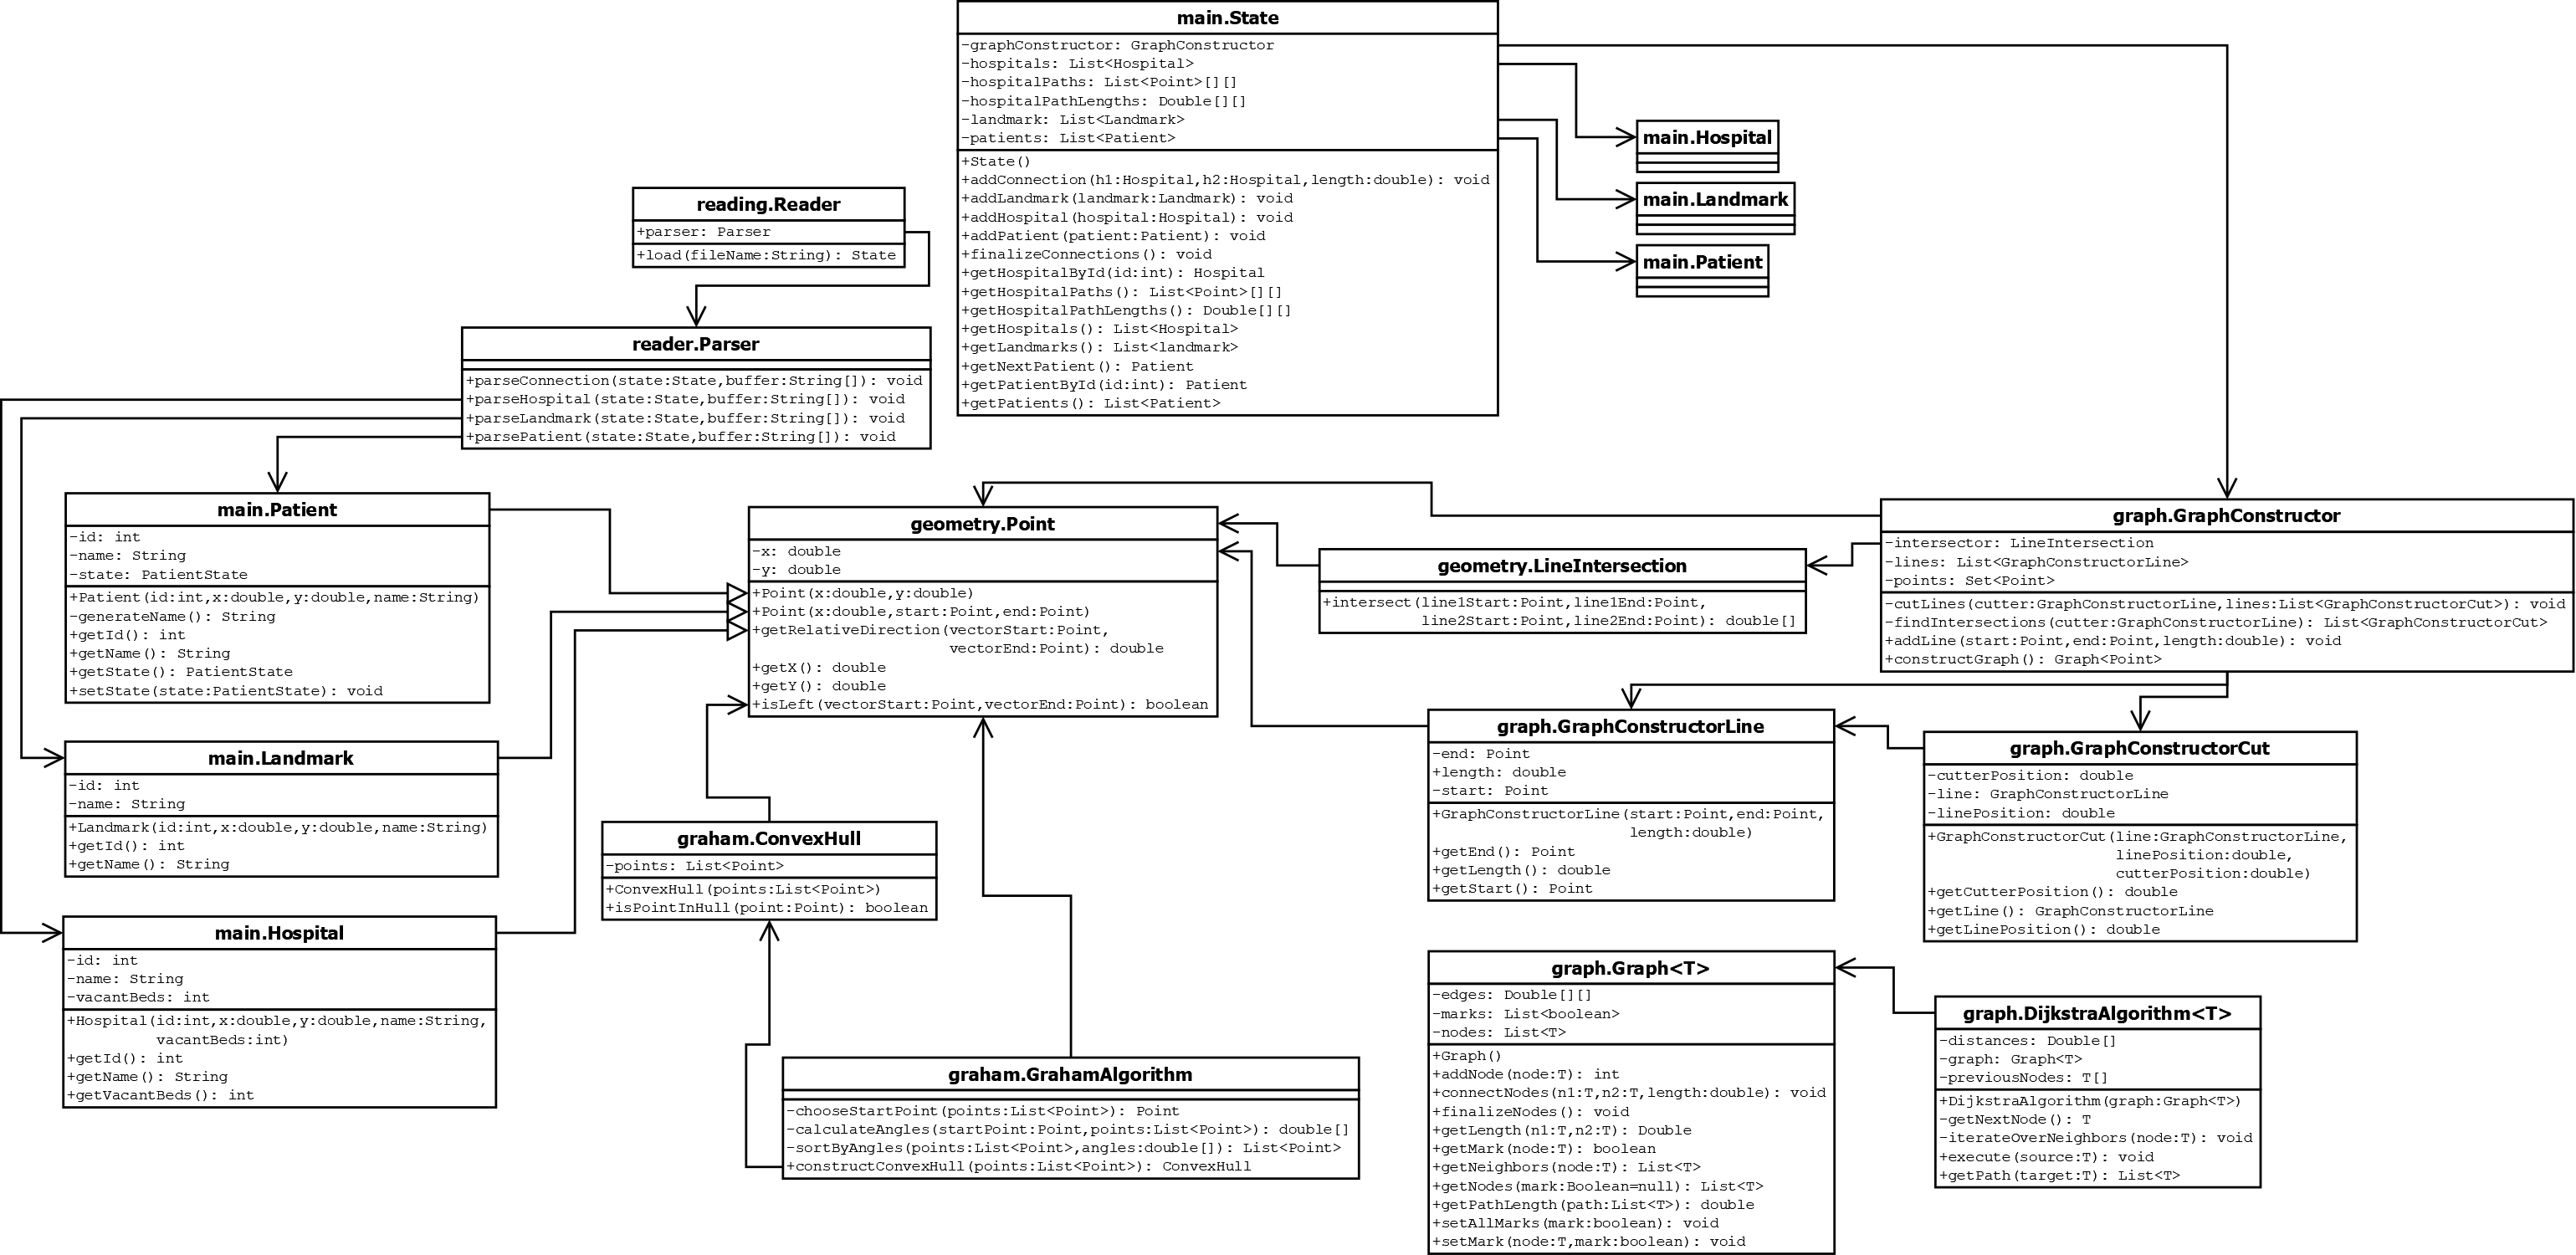
\includegraphics[scale=0.15]{images/UML.png}
    \caption{Diagram UML klas projektu.}
\end{figure}
\end{landscape}

\section{Testowanie}
Do testów jednostkowych wykorzystamy narzędzie JUnit 5.
Program jest złożony, wykorzystuje kilka oddzielnych algorytmów, dlatego staramy się jak najdokładniej przetestować każdy z nich. Za działanie każdego algorytmu odpowiedzialnych jest kilka/kilkanaście metod, które chcemy szczegółowo przetestować. Graficzny interfejs użytkownika testować będziemy podczas pisania programu. Po każdej operacji związanej ze zmianą wyglądu gui będziemy sprawdzać, czy zmiana nastąpiła prawidłowo, a także czy wszystkie dane są widoczne i czytelne.

\subsection{Warunki brzegowe}
Podczas testowania musimy zwrócić szczególną uwagę na następujące przypadki:

\begin{itemize}
    \item czy klasa \texttt{reading.Parser} prawidłowo rozpatruje wszystkie możliwe błędy, czy wyświetla się stosowny komunikat
    \item w klasie \texttt{graham.ConvexHull} należy sprawdzić, czy metody dobrze obliczają kąty i prawidłowo je sortują, a także czy położenie wszystkich obiektów jest brane pod uwagę przy wyznaczaniu otoczki wypukłej
    \item  czy metoda \texttt{isLeft()} z klasy geometry.Point za każdym razem prawidłowo określa położenie punktu względem wektora
    \item czy proporcje odcinków po przecięciu są prawidłowo obliczane w klasie graph.GraphConstructorLine
     \item czy klasa \texttt{graph.DijkstraAlgorithm<T>} bierze pod uwagę wszytskie możliwe połączenia(nie pomija żadnych dróg)
    \item czy w klasie \texttt{graph.DijkstraAlgorithm<T>} prawidłowo jest określana długość dróg i czy w każdym przypadku wybierana jest najkrótsza z nich
    \item czy klasa \texttt{graph.GraphConstructor} korzysta ze wszystkich dostępnych skrzyżowań  (przecięć dróg między szpitalami)
\end{itemize}

\subsection{Warunki brzegowe dla graficznego interfejsu użytkownika}
\begin{itemize}
    \item czy lista szpitali/pacjentów jest na bieżąco aktualizowana
    \item czy sekcja informacyjna jest aktualizowana, czy wyświetla prawidłowe informacje
    \item czy podczas manualnego dodawania pacjenta współrzędne jego położenia są prawidłowo określane i wczytywane
    \item czy mapa jest poprawnie załadowana, widoczna w całości (odpowiednie wyskalowanie), punkty na mapie są podpisane i czytalne, a oznaczenia symbloliczne i kolorystyczne poprawne
\end{itemize}

\end{document}
